
\section{Derivable functions can be described in first-order logic}
\label{sec:to-logic}
We show in this section that derivable functions can be implemented by first-order transductions. The proof proceeds by induction, following the definition of derivable functions. All the cases are easy, and consist mainly on unfolding the definitions. We will treat only the cases of the basic function $\unit_\rSigma$  to illustrate this process.
    
    In the following, it will be convenient to use, as part of the vocabulary of $\rSigma$, the unary relation  $\mathsf{Port}_\rSigma$ which selects the ports of the structures over the vocabulary of $\rSigma$; and the binary relation $\sqsubset_\rSigma$ which orders these ports. By induction on $\rSigma$, we can show that both relations are definable by first-order formulas over  the vocabulary of $\rSigma$.
    
    
   Given an element $x$ of $\rSigma$, let us show how  $\unit_\rSigma(x)$ can be implemented using a FO transduction.  The copying constant is 2,
    the first copy will contain the whole structure $\underline{x}$ and the second copy will select only the ports of $\underline{x}$ which will serve as the ports of the structure $\underline{\unit_\rSigma(x)}$, as illustrated by the following picture 
\begin{center}
    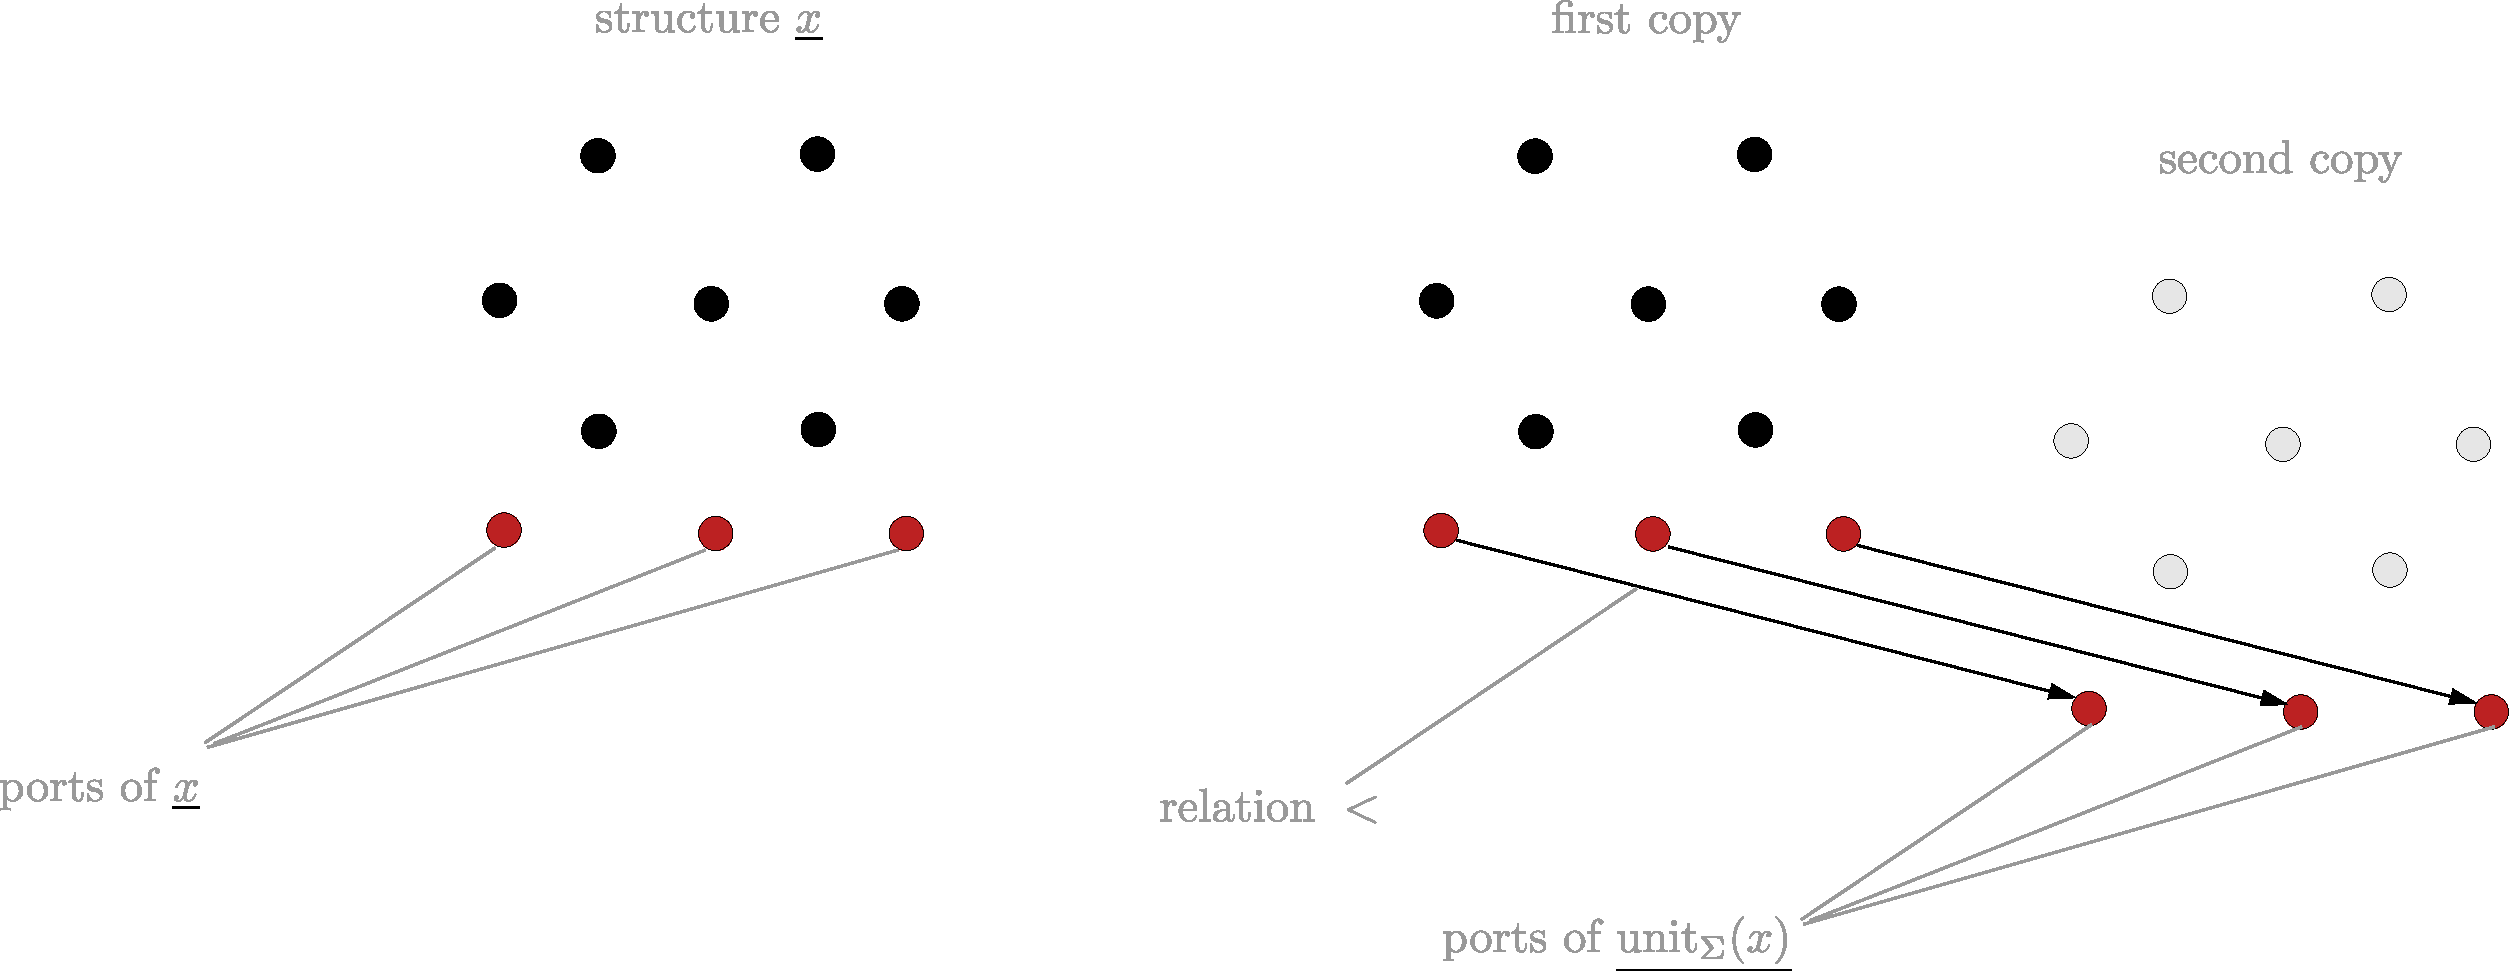
\includegraphics[scale=.3]{to-logic-unit.pdf}
    \end{center}    
      The universe formulas are then:
    \begin{align*}
    \varphi_1(x)=\mathsf{True} \qquad \varphi_2(x)=\mathsf{Port}_\rSigma(x)
    \end{align*}
    In the first copy, the vocabulary of $\rSigma$ will be interpreted as in the original structure, and as the empty set in the second copy. That is, for every unary relation $R$ and for every binary relation $S$ in the vocabulary of  $\rSigma$, we set:
    \begin{align*}
   \varphi_R^{1}(x)=R(x) \quad&\quad \varphi_S^{1,1}(x,y)=S(x,y)\\
   \varphi_R^{2}(x)=\mathsf{False} \quad&\quad \varphi_S^{2,2}(x,y)=\mathsf{False}
\end{align*}      
Let us interpret the relations $<$ and $\sqsubset$ of the vocabulary of $\tmonad\rSigma$. The  ports of $\underline{\unit_\rSigma(x)}$ inherit the order of the ports of $\underline{x}$, this is why we set:
\begin{align*}
\varphi_\sqsubset^{2,2}(x,y)=x\sqsubset_\rSigma y
\end{align*}
The descendant relation $<$ connects the $i^{th}$ port of $\underline{x}$ to the $i^{th}$ port of $\underline{\unit_\rSigma(x)}$. Since these nodes come from the same node in the original structure, we set:
\begin{align*}
\varphi_<^{1,2}(x,y)=x=y
\end{align*}